\message{ !name(Rapport.tex)}\documentclass[12pt]{article}
\usepackage{style}
\usepackage{hyperref}
\usepackage{float}
\newcolumntype{L}[1]{>{\centering\let\newline\\\arraybackslash\hspace{0pt}}m{#1}}
\newcolumntype{C}[1]{>{\centering\let\newline\\\arraybackslash\hspace{0pt}}m{#1}}
\newcolumntype{R}[1]{>{\centering\let\newline\\\arraybackslash\hspace{0pt}}m{#1}}
\title{
\includegraphics[scale=1]{store_logo}\\Tredie Delrapport \\ Projektgruppe-id: A6}
\author{Tobias Hallundbæk Petersen - 081092\\Nikolaj Dybdahl Rathcke - 180692\\ Ola Rønning - 200190\\ Victor Petrén Bach Hansen - 130892 \\\\ Instruktor : Andreas Frisch}
\begin{document}

\message{ !name(Rapport.tex) !offset(-3) }

\maketitle
\newpage
\tableofcontents
\newpage
\section{Abstract}
We are making an Android application for the company eBogreolen.dk. This application needs features that enables their customers to search for e-books and audiobooks. The application should make the users able to buy e-book and audiobooks. This means that there needs to be a payment method for the e-books and audiobooks. Additional features, if possible, would be to implement a way of reading the e-books and hearing audiobooks though this is not a requirement for the finished product.\\
More specifically, the functional requirements of the project described with different diagrams. It discusses the user interface with screens of the user interface as well as a description of the interaction between the user and the application.\\
The language for developing for Android is Java, therefore this is the language that will be used in the development of the application, the application will furthermore be developed for all Android platforms of version 2.3 or higher.\\
The application will get the content from eBogreolen.dk and the owners of that site will take care of adding and maintaining content, this entails that the application must keep itself up-to-date with the content of the eBogreolen.dk's database.

\section{The purpose and constraints of the IT-solution}
This is based on the FACTOR-concept, and explains the scope of the project.
\paragraph{Functionality}
\begin{enumerate}
\item A way of buying and paying for books.
\item Ability to download and use the bought books.
\item A search and browse functionality.
\end{enumerate}

\paragraph{Application domain}$ $\\
The application domain is Android phone users who are customers at eBogreolen.dk.
\\
\paragraph{Conditions}$ $\\
The specification of android devices vary greatly and the application should run evenly on all devices.
\\
\paragraph{Technology}$ $\\
The system will be developed entirely in Java with the Android SDK and will be run on Android smartphones with Android version 2.3 or higher.
\paragraph{Objects}
The objects of the Application are the Ebooks, Audiobooks, an online bookshelf, and a user account.
\\
\paragraph{Responsibility}$ $\\
Making the user able to browse, buy, read and listen to ebooks and audiobooks.
\section{Requirements specification}
This section explains what is to be expected of the application when it is completed, furthermore it also specifies different use cases and the problems that might appear.
\subsection{Functional and Non-functional requirements}

Functional requirements:
\begin{enumerate}
\item Login capability.
\item Purchase ebooks and audiobooks in the Android application.
\item Show purchased ebooks and audiobooks in an account specific bookshelf.
\item Download purchased ebooks and audiobooks available from the eBogreolen website.
\end{enumerate}
$ $\\
Non-functional requirements:
\begin{enumerate}
\item Stability and reliability. We need a stable application, for example, to make sure all transactions are atomic.
\item Usability. We want to make sure that the application is as easy and intuitive as possible, for the best costumer experience.
\item Security. Since we are dealing with others peoples money, we will need a secure system.
\item An offline-mode, for reading books when not connected to the internet.
\item The application should run on its own, and no administration should be needed.
\end{enumerate}

\subsection{Casemodel}

The casemodel shown in figure \ref{casemodel}, shows what different cases the user can experience using the Android application. This is a rather simplified diagram, showing the key features that a user will experience.
\begin{figure}[H]
\center
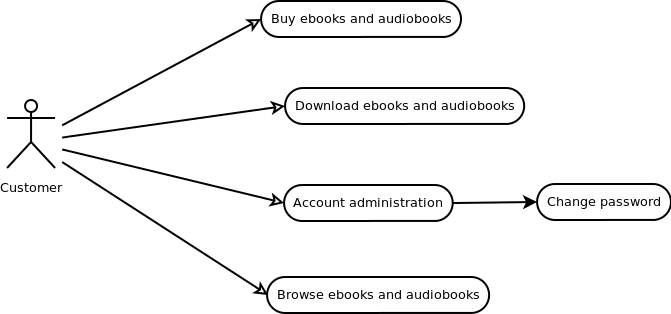
\includegraphics[scale=0.7]{Casemodel.png}
\caption{A case model describing the use cases of the Application.}
\label{casemodel}
\end{figure}

\subsection{Usecases}

\begin{enumerate}
\item 
Title: Logging in\\
Main Success Scenario:\\
  Step 1: The user presses the log in button.\\
  Step 2: Then the user enters his/her username and password.\\
  Step 3: He/she then submits the information by pressing a button.\\
  Step 4: His/her books are now loaded to the application, as paths to the locally downloaded book.\\
Extensions:\\
  Extension 2a: The user writes a wrong username and/or password.\\
  Extension 3a: There is no internet connection.\\
\item 
Title: Buying book\\
Main Success Scenario:\\
  Step 1: The user presses the buy button.\\
  Step 2: Then the user enters his/her credit card details.\\
  Step 3: He/she then submits the information by pressing a button.\\
  Step 4: The book is added to the users account.\\
Extensions:\\
  Extension 2a: The user writes wrong card details.\\
  Extension 3a: There is no internet connection.\\
  Extension 3b: The transaction was denied.\\
\item 
Title: Search for a book\\
Main Success Scenario:\\
  Step 1: The user presses the search bar.\\
  Step 2: A search query is written.\\
  Step 3: The query is committed.\\
  Step 4: The results are shown.\\
  Step 5: A book is chosen.\\
Extensions:\\
  Extension 3a: There is no internet connection.\\
  Extension 4a: The query returned no books.\\
\end{enumerate}
\subsection{Class diagram}
The class diagram shown in figure \ref{uml}, describes the outline of the solution-domain. This is not the final design, as there are many uncertainties, which is described in depth in section \ref{sec:Syssum}.
\begin{figure}[H]
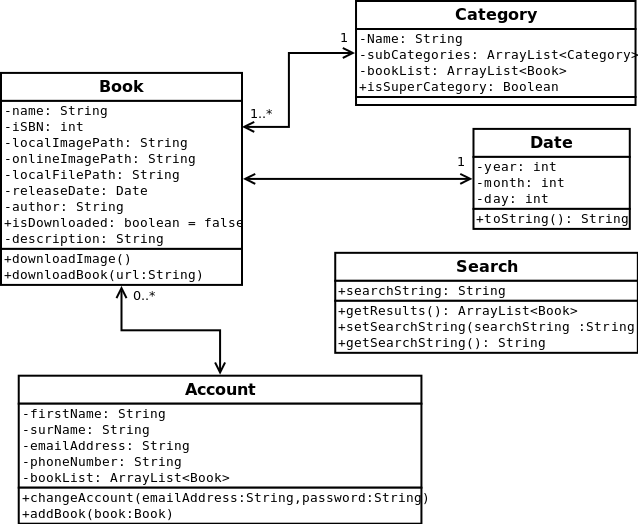
\includegraphics[scale=0.6]{uml.png}
\caption{A uml diagram over the Application}
\label{uml}
\end{figure}
\subsection{Sequence diagrams}

The sequence diagram shown in figure \ref{SeqDiaLogin} shows the chain of inner workings that is executed when the user tries to log in.
\begin{figure}[H]
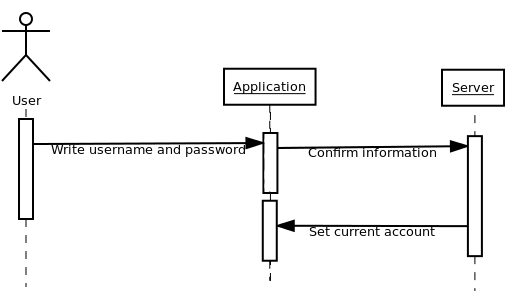
\includegraphics[scale=0.6]{SequenceDiagramLogin.png}
\caption{A sequence diagram for when a user logs in}
\label{SeqDiaLogin}
\end{figure}

The sequence diagram shown in figure \ref{SeqDiaBuyBook} shows the chain of inner workings that is executed when the user tries to buy a book.
\begin{figure}[H]
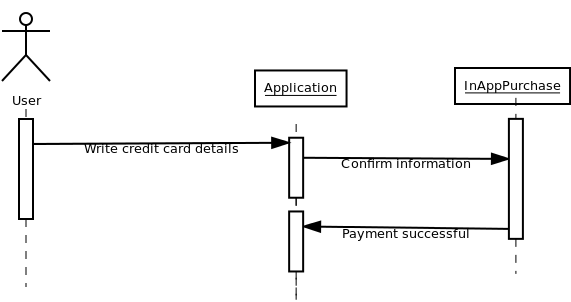
\includegraphics[scale=0.6]{SequenceDiagramBuyBook.png}
\caption{A sequence diagram for when a user buys a book}
\label{SeqDiaBuyBook}
\end{figure}

The sequence diagram shown in figure \ref{SeqDiaBookSearch} shows the chain inner workings that is executed when the user tries to search for books.
\begin{figure}[H]
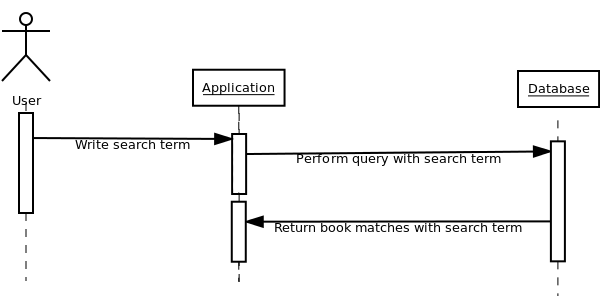
\includegraphics[scale=0.6]{SequenceDiagramBookSearch.png}
\caption{A sequence diagram for when a user searches for a book}
\label{SeqDiaBookSearch}
\end{figure}

As you may notice, the sequence diagrams have no backflow, this is due to the fact that the application must maintain itself, as no administration should be needed, other than what is performed to the eBogreolen.dk website, and the associated database.

\section{Systemdesign summary}
\label{sec:Syssum}
As of right now, the system is a number of classes and methods that was foreseen would be needed in the final design of the back end of the android application. Further we are developing the front end, with dummy functionality to be ready for the WebAPI that EBogreolen will have finished for us in week 18. When we have the WebAPI we will finish the back end and then look to find payment solutions as discussed below.
\\\\
Some of the most important remaining design and implementation task are as follows:
\\\\
GUI:\\
We have now started the development of the GUI, we are using the design drawn, see figures \ref{Front page}, \ref{Book information}, \ref{Categories}, \ref{Results}, by the group as guide to the final look and feel of the GUI. Before starting the front end development the group discussed in detail how each of the pages should be understood. These discussions are summarized in a set of pictures annotated with our conclusions, see figure \ref{Table0}, \ref{Table1} and \ref{Table3}.
\\\\
\begin{figure}
 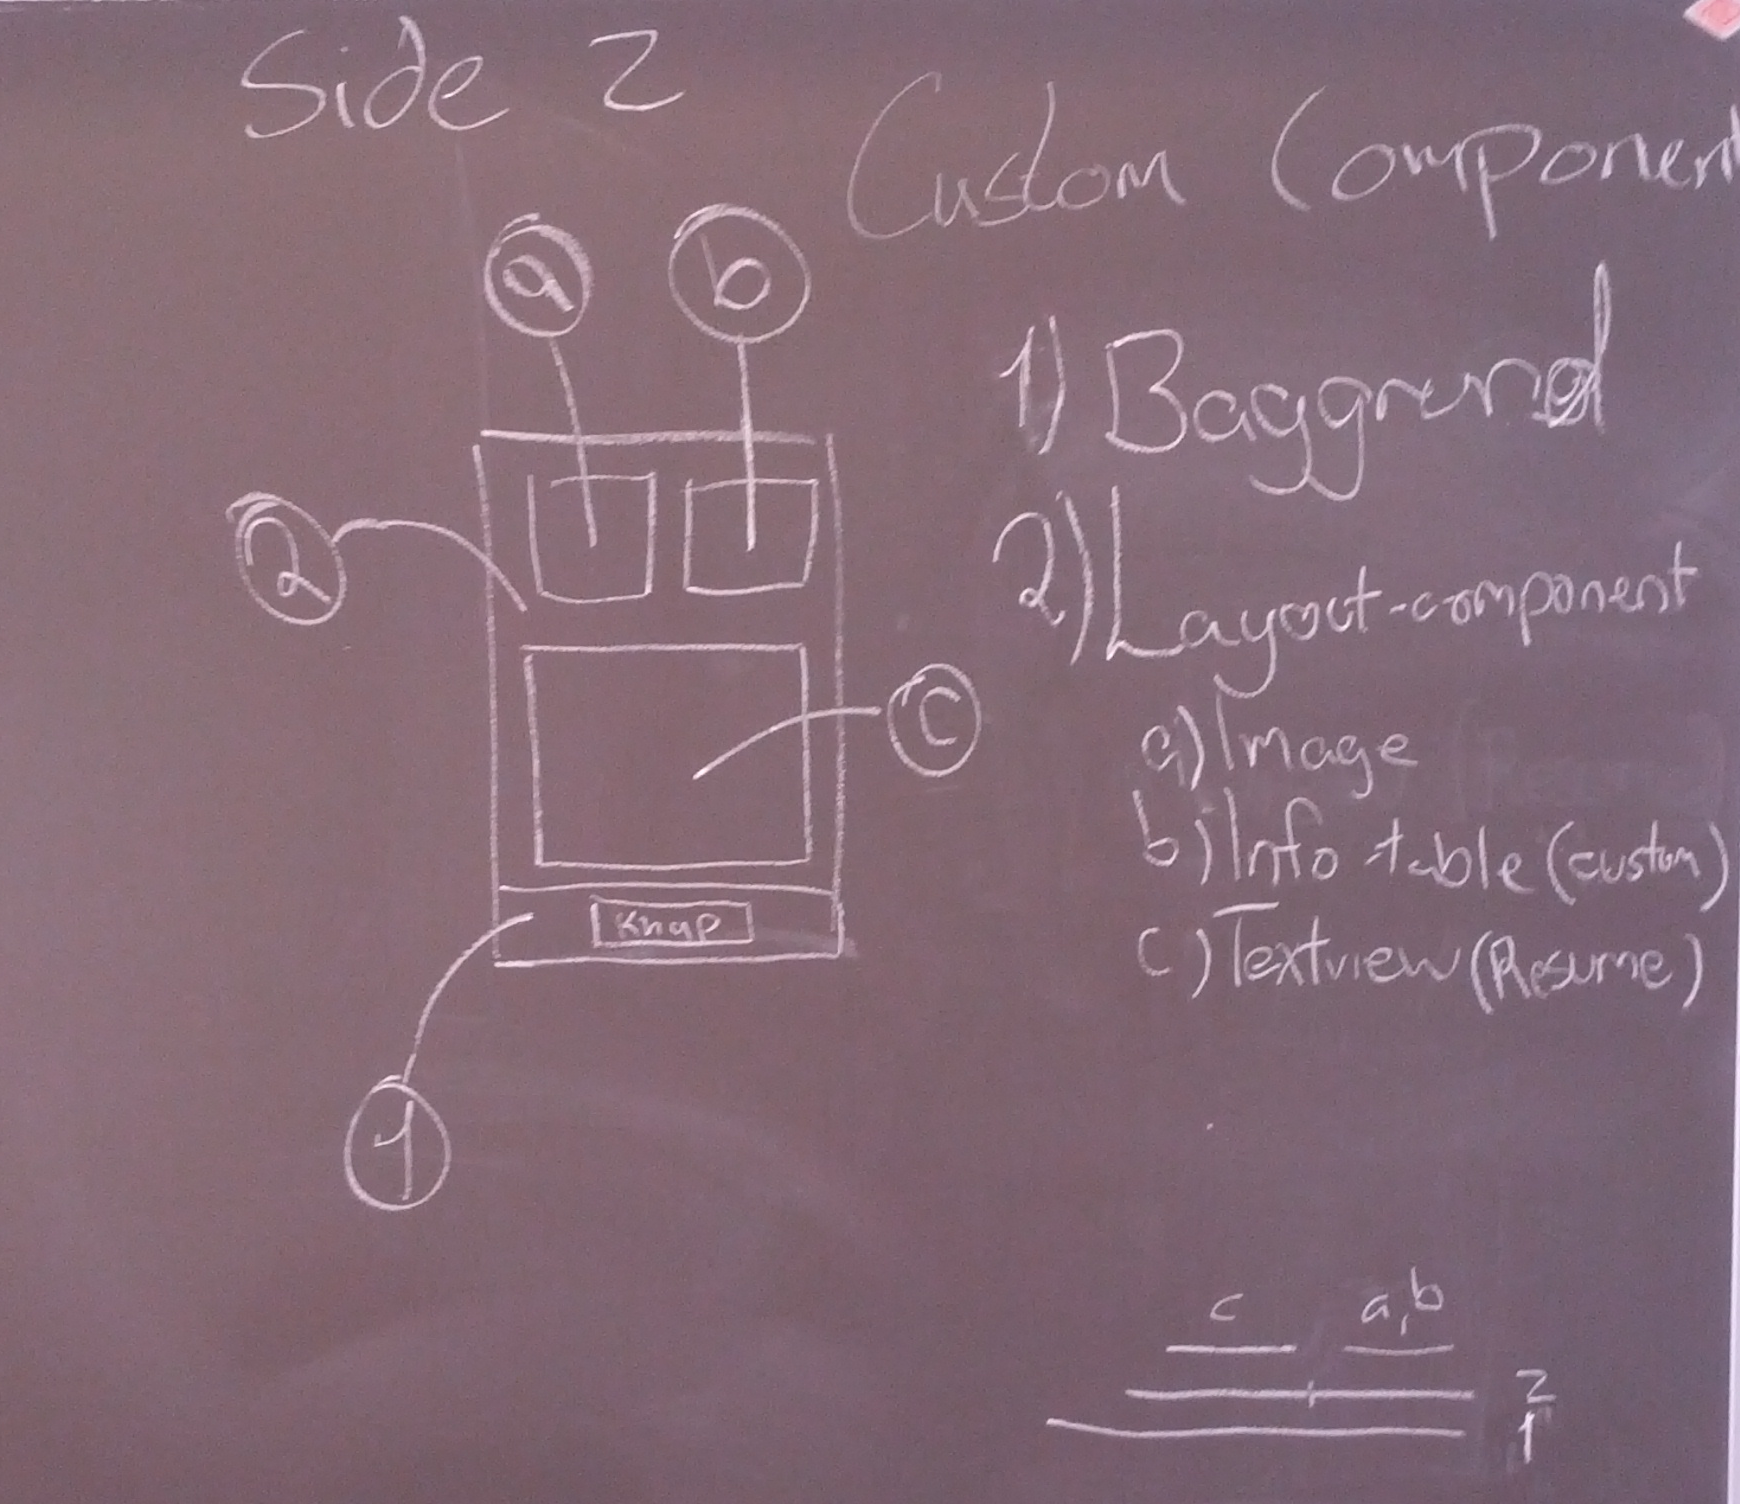
\includegraphics[scale=0.2]{Tavle}
\caption{ }
\label{Table0}
\end{figure}
\begin{figure}
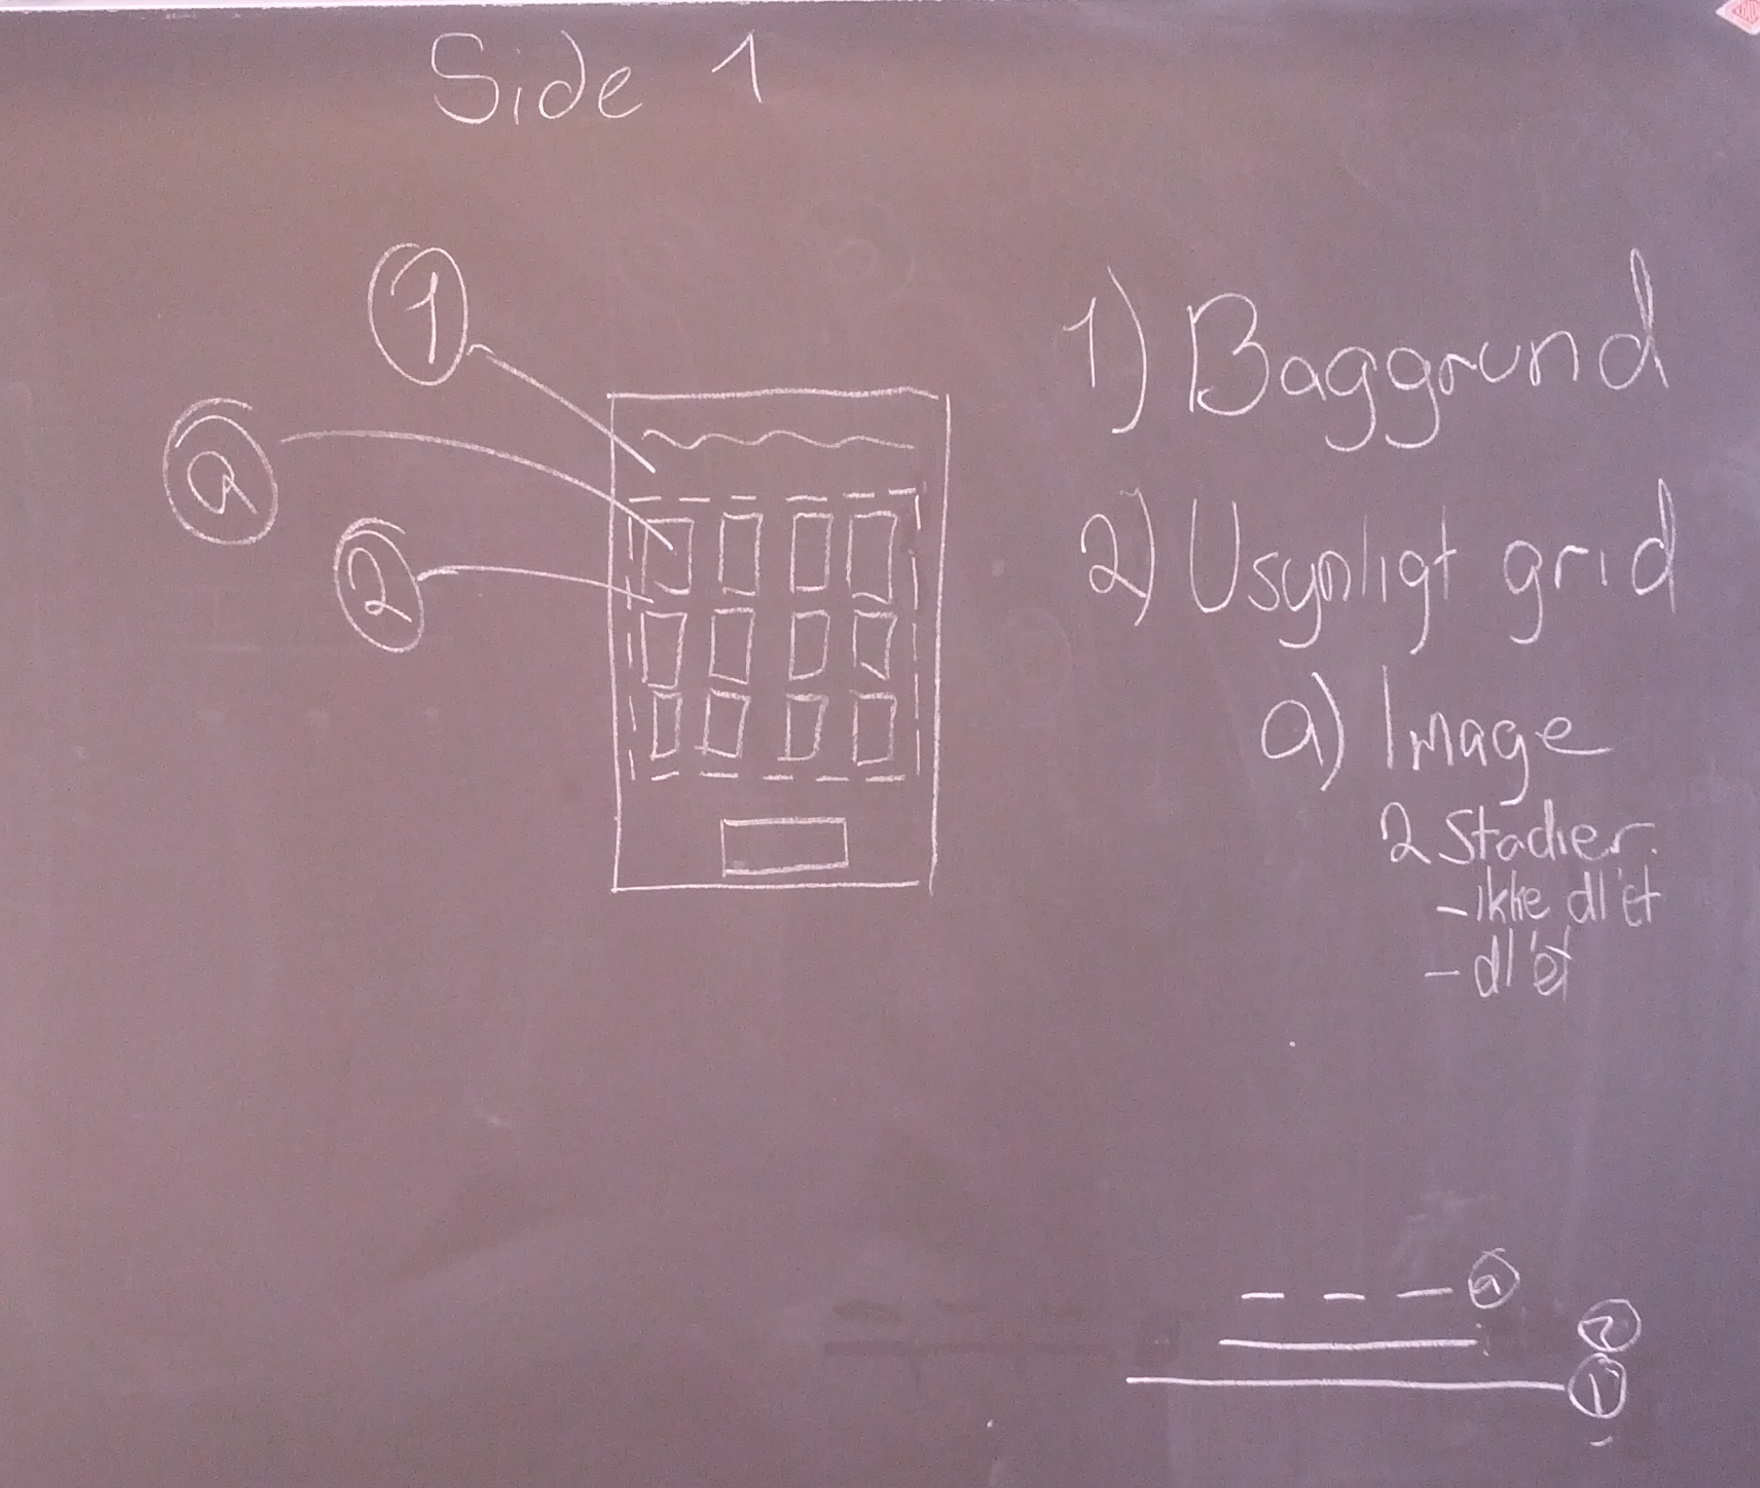
\includegraphics[scale=0.2]{Tavle1}
\caption{ }
\label{Table1}
\end{figure}
\begin{figure}
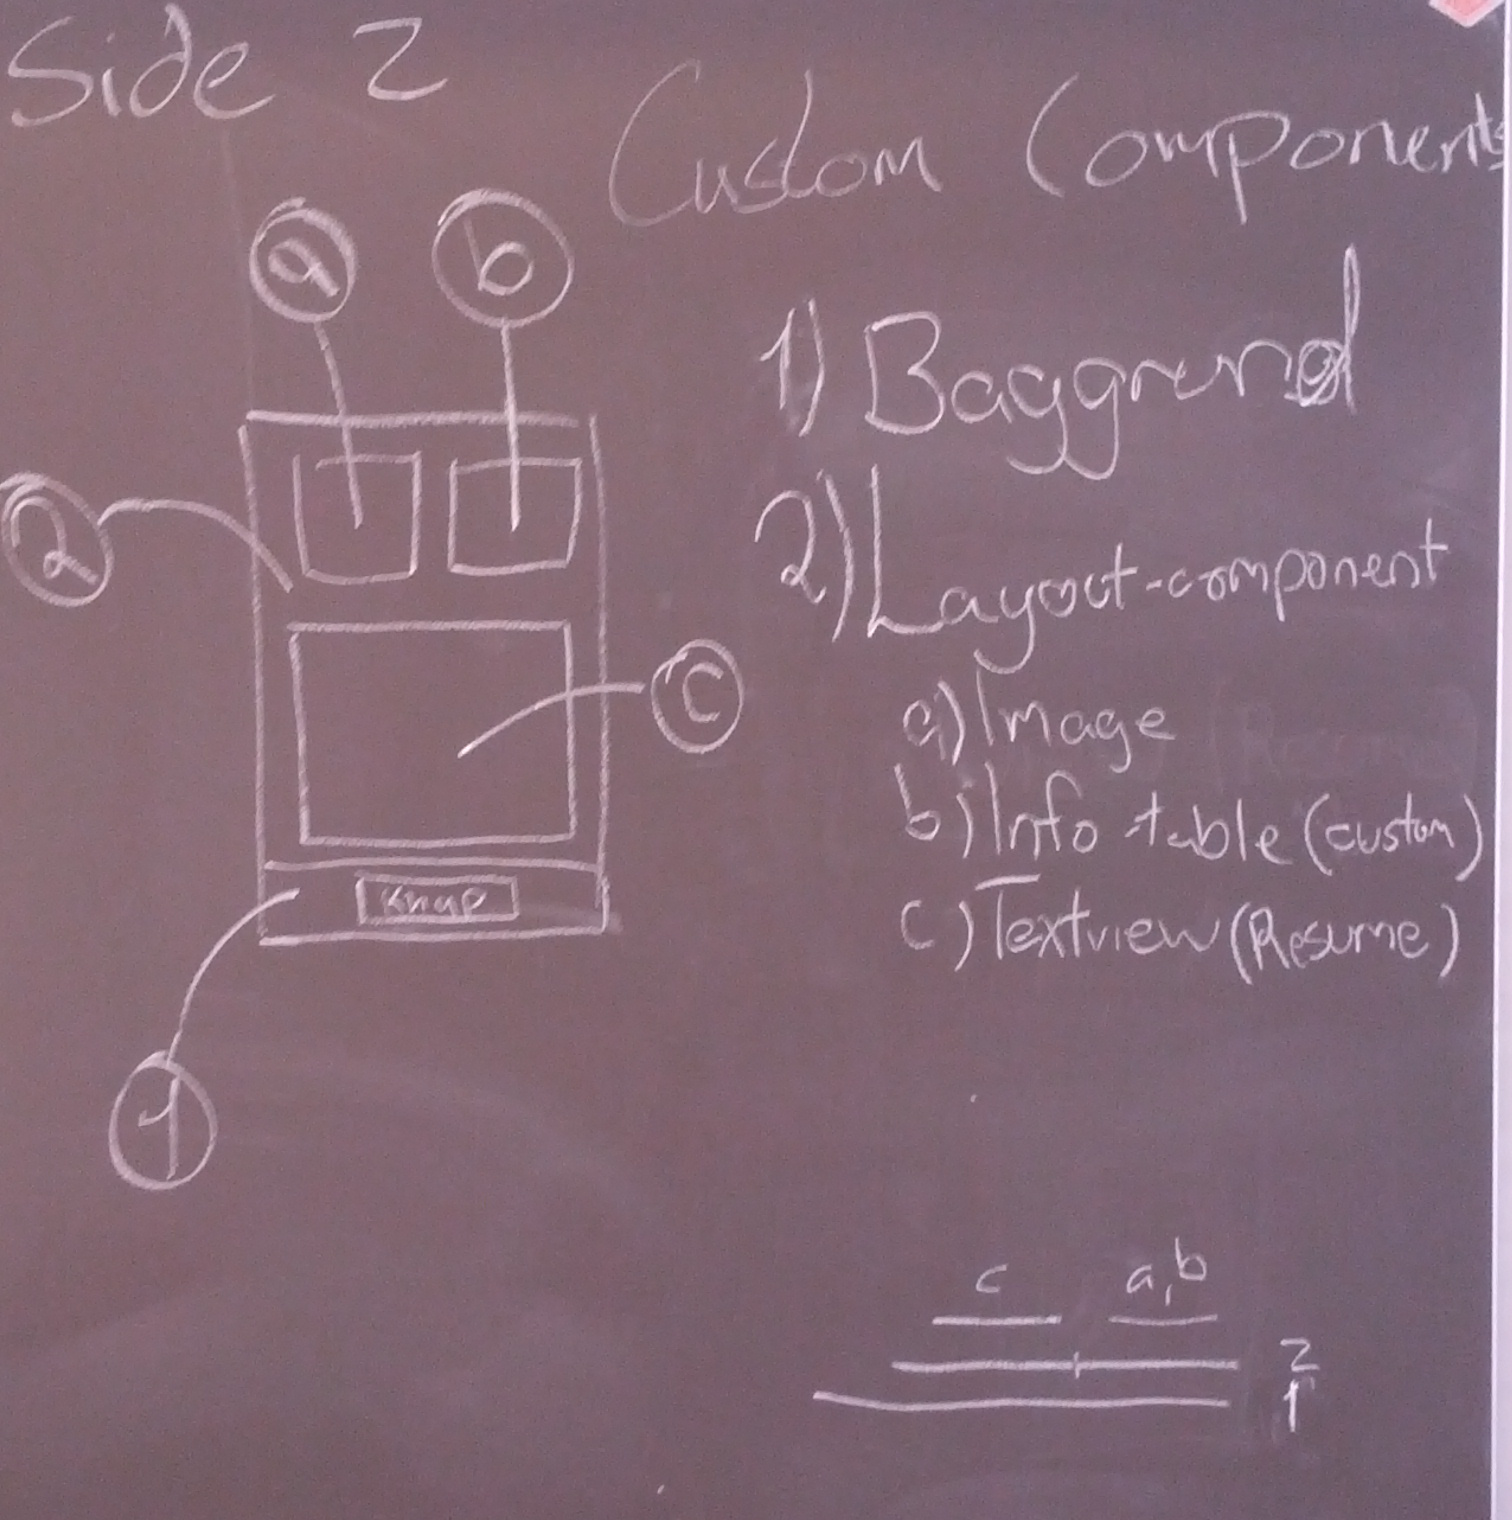
\includegraphics[scale=0.2]{Tavle3}
\caption{ }
\label{Table3}
\end{figure}
A payment solution:\\
When a customer wants to buy a book, the system for handling this is needed. The Android SDK provides a tool for this, but it has yet to be implemented and fully understood.
\\\\
The WebAPI:\\
This will be implemented by eBogreolen.dk's developer Anders Hyldig and will facilitate the interaction with the database. We now have conformation that this webAPI will be finished in week 18, with the following functionality:
\begin{enumerate}
\item Pulling of books.
\item Pulling of single book with further detail.
\end{enumerate}
Database interaction:\\
The queries that the user makes regarding bought books and browsing for new books needs to be taken care of, the implementation of this depends on the WebAPI. This will be the focus of the next sprint which will start once we have the webAPI.
\section{Program and system test}
\label{systest}
Since we do not have a functional application as of this moment, no actual tests have been performed yet. We plan to, as soon as possible, to construct a pen and paper version of our desired interface, which we will use for a series of think-out-loud tests, to determine the usability of our design. These tests will be performed on people, who will have no relation to neither us nor the project, but rather random people who happen to agree to be subjected to them.\\
We will, as soon as we get a working dummy-prototype up  and running, perform the same tests once more in order to get the most satisfying results. We have deemed this appropriate as the Android Application market, along with our client, has a wide range of users.\\ \\
A JUnit testsuite is yet to be established, but is still a work in progress in the process of testing the backend of our Java code.
\section{Userinterface and interaction design}
The external interfaces are here understood as the finished product GUI, for which we have a course outline as it follows in Figure \ref{Front page},\ref{Book information},\ref{Categories} and \ref{Results}. The application GUI for the login page has not been developed yet.
\begin{SCfigure}
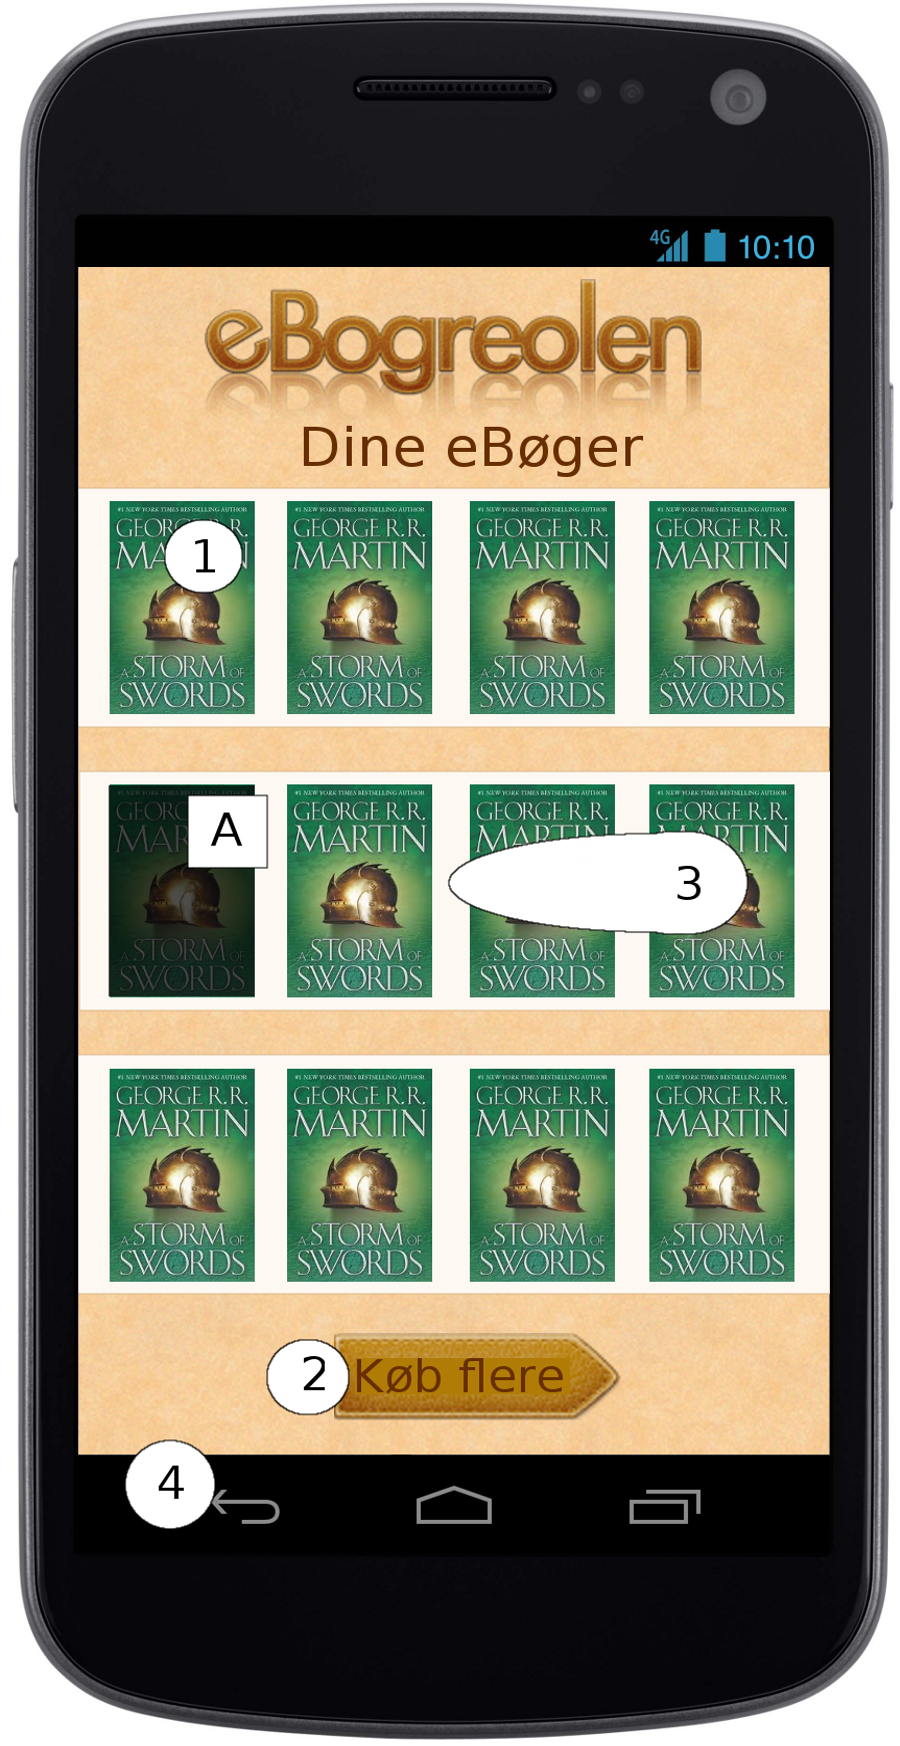
\includegraphics[scale=0.7]{gnexforside.png}
\caption{
\\
1. Open a page containing the information of a purchased book. This will lead to Figure \ref{Book information}.\\\\
2. Search/browse after more books to purchase. This will lead to Figure \ref{Categories}.\\\\
3. Swipe to the side to look at more of your books.\\\\
4. This button will always go one page back. If there are no more pages to go back to, the application will be closed.\\\\\\
A. This book is darkened, because the book has been purchased, but not downloaded.
}
\label{Front page}
\end{SCfigure}

\begin{SCfigure}
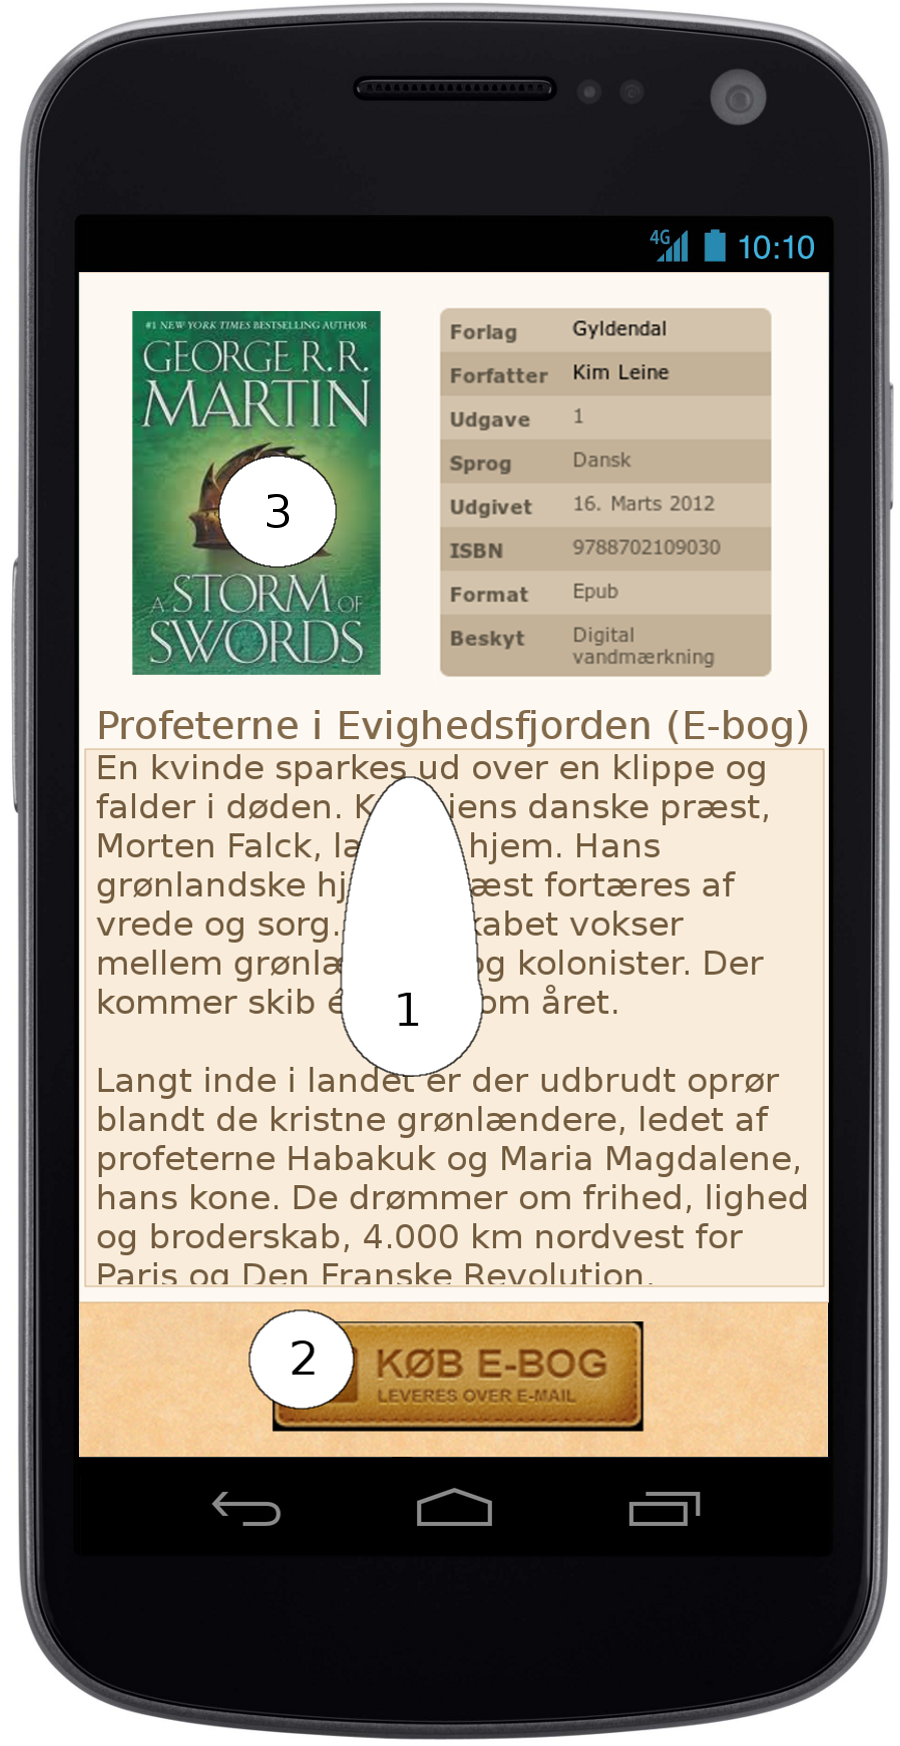
\includegraphics[scale=0.7]{gnexinfodownloadogkoeb.png}
\caption{
\\
1. Swipe up and down to read a description of the book.\\\\
2. This button can be a: Buy, Download, Read or Listen button, this depends on whether or not you own the material and/or if its an audiobook or ebook.\\\\
3. Tapping the image enlarges it to a full screen view, tapping the image while enlarged will return to the displayed page.
}
\label{Book information}
\end{SCfigure}
\begin{SCfigure}
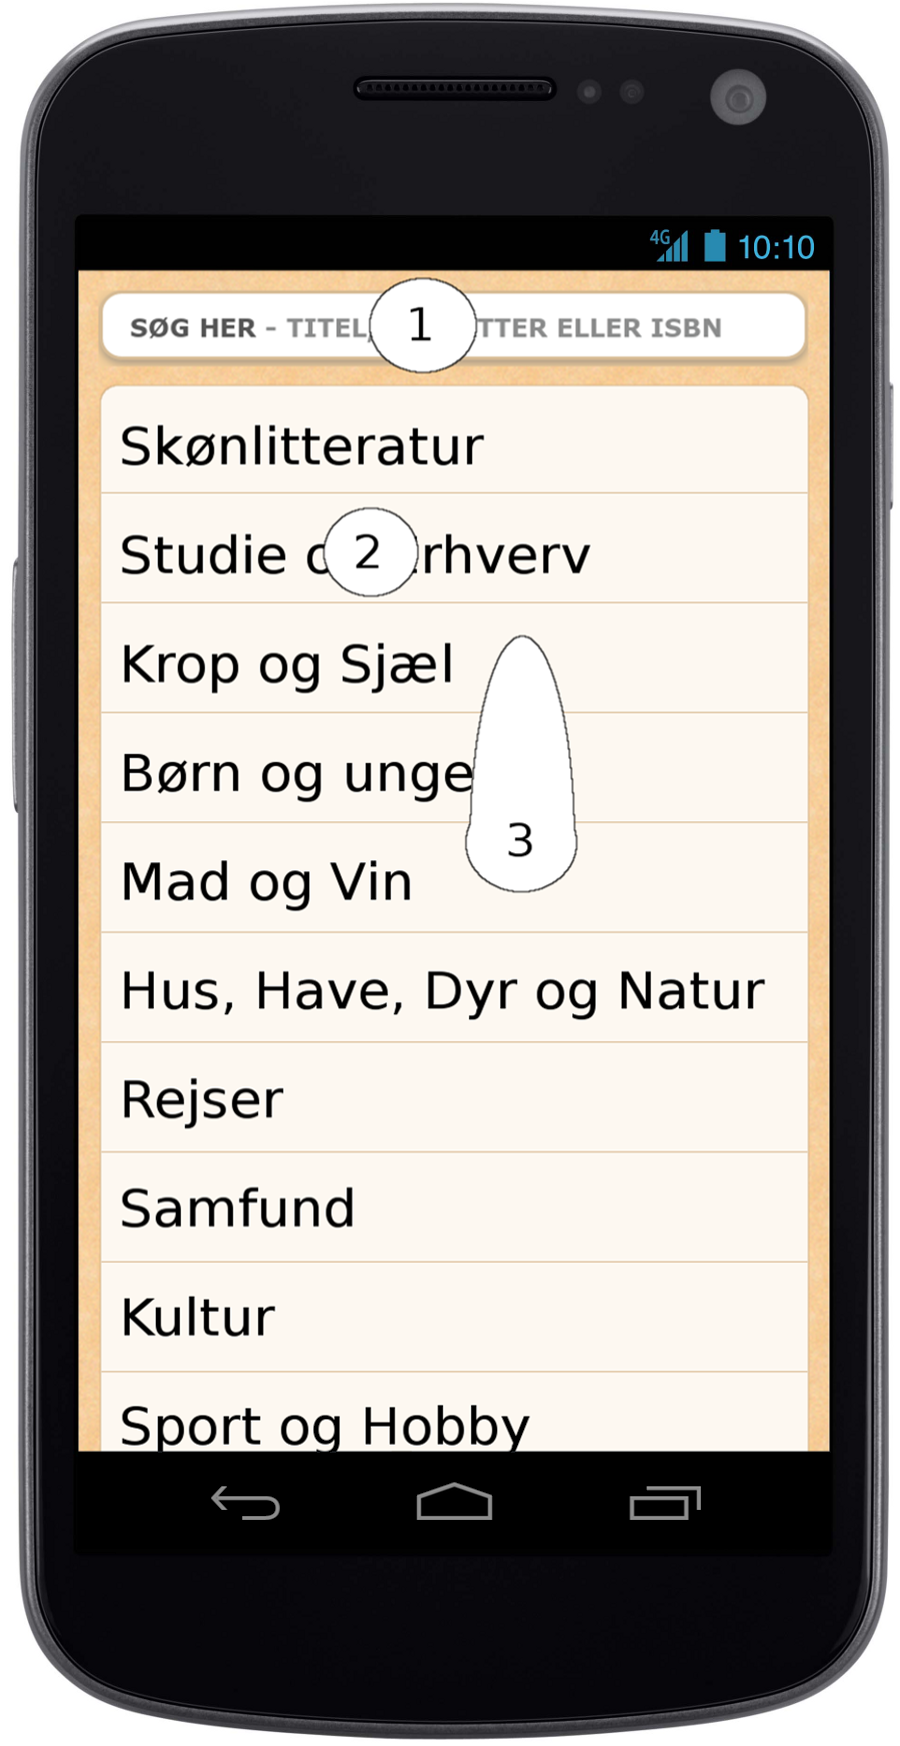
\includegraphics[scale=0.7]{gnexsoegeogbrowse.png}
\caption{
\\
1. This will access the search function, when a search is complete it will direct you to Figure \ref{Results}\\\\
2. The will open the category in this interface if it is a super category, and go to Figure \ref{Results} it is a sub category.\\\\
3. Swipe up and down to browse the categories.
}
\label{Categories}
\end{SCfigure}

\begin{SCfigure}
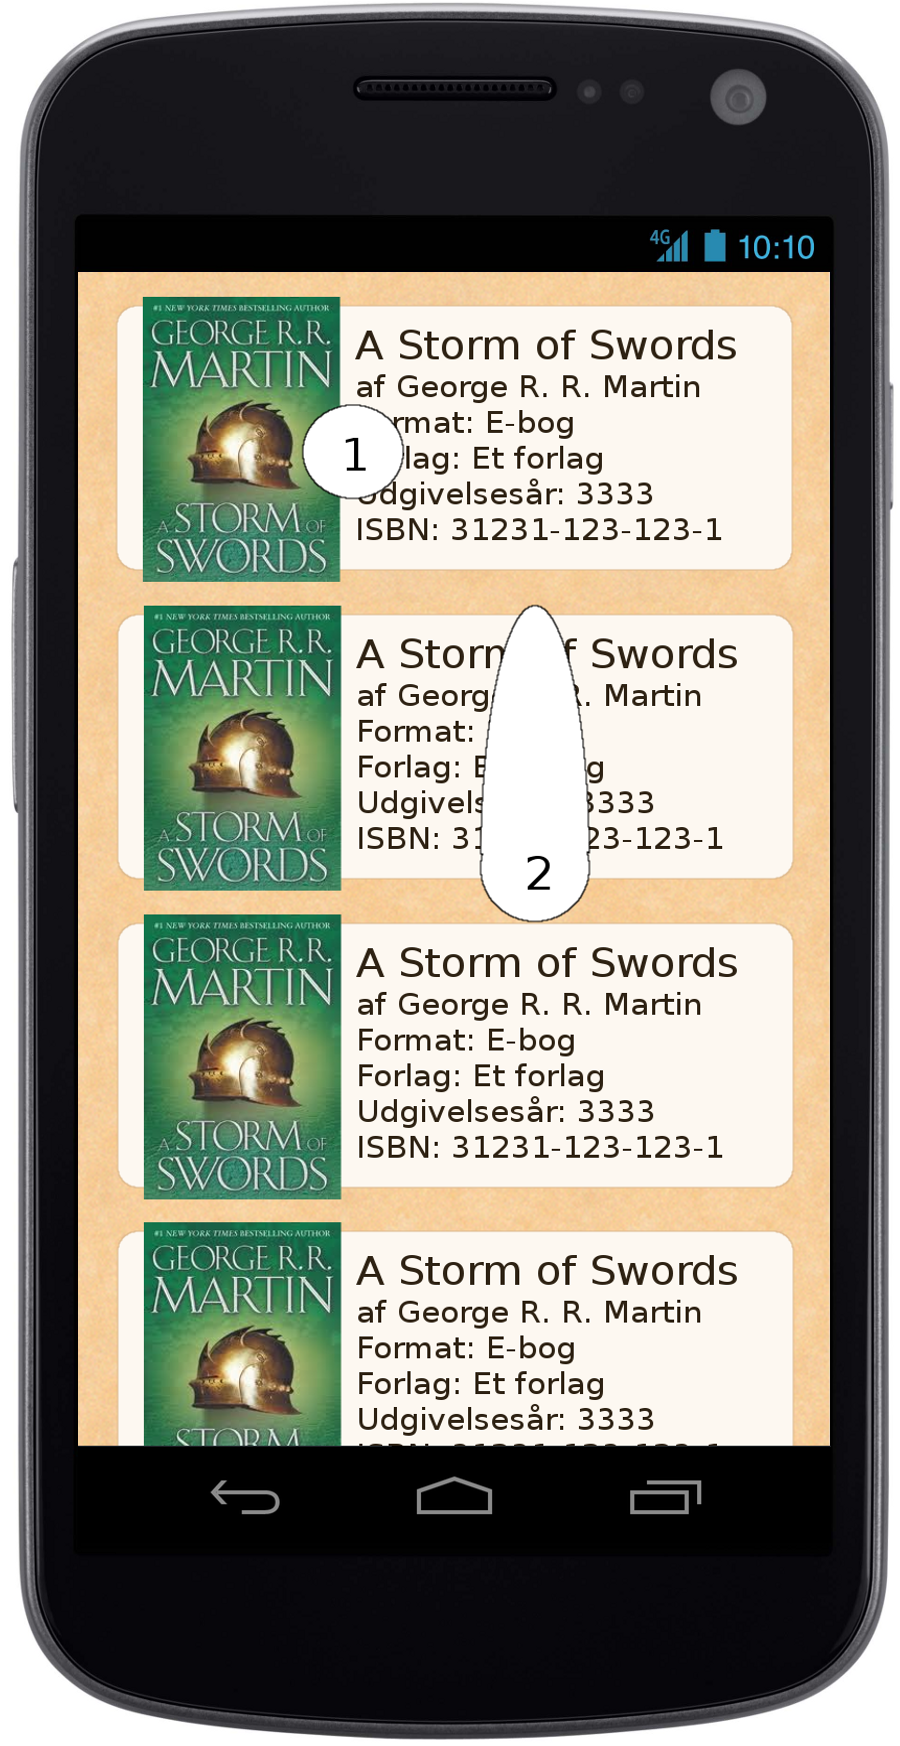
\includegraphics[scale=0.7]{gnexresultater.png}
\caption{
\\
1. This will take you to the information of the given book, this will lead to Figure \ref{Book information}.\\\\
2. Swipe up and down to browse the results.
}
\label{Results}
\end{SCfigure}

\subsection{Audio-visual presentation}
On this stage we do not have a prototype of our product, but the final product is expected to look like what's given in section 6.1, therefore an audio-visual presentation would be pointless.

\subsection{Latest think-out-loud results}
As described in section \ref{systest}, a think-out-load test has not yet been performed, and therefore no results are present.
\newpage
\section{Versioncontrol}

The following is the commitlog for our repository at https://github.com/VixQIT/EBogreolen where our code is accessible as well:
\begin{verbatim}
$ git log --pretty=oneline

eec27a1012dcf399187a98ad42de842d Fix of your books activity
96927130e41cf1f71b08aea0578cd424b3c0c9a7 Setup of android app environment, and a
258566b216827dd09a6186042069f4ecb563faf5 Merge branch 'master' of https://github
5176586754383ad696ecc8da6e3b1a089b611ad1 First commit
86bf9e9a7090a87a986ecf6bf7ec34ed094a56f7 Initial commit
\end{verbatim}
Since the first and initial commit, the classes and XML layout styles have been added to the code. Furthermore the classes that were committed in the first commits have been merged into the code structure, these classes are still unused as we have no actual data to work with. Dummy data in the form of book covers has been added as well. The code added forms an outline of the GUI first showed in Figure \ref{Front page}. More code that implements the GUIs described in Figure \ref{Book information}, \ref{Categories} and \ref{Results} have been more or less developed and will be committed once the code is fully functional with the prior code. A clone of the repository will now yield a the code for an application that can be run on any Android device of version 2.3 or higher, though a path for a local ADK must be provided, and some other system specific settings. Furthermore it will hold the most updated working application.

\section{Project collaboration}
We have developed a 'game' using 'experience' points and the opportunity to 'level' up. These point are distributed to the group participants by a point generator on: \url{http://www.VixQIT/XP/XP.php}
that generates a random amount of point in a certain range. The range is calculated from tasks completed. Tasks are worth points equal to the hours of work estimated during our scrum and these translates into points that provides the range from your random gain of experience.\\
The experience needed to level up increases each time using the Fibonacci sequence.\\
This game a motivation for us since there are small benefits (bragging rights, beers etc.) and the idea of making it competitive is appealing to all of us. While keeping the simple benefits, it won't ruin the dynamics in the group. Keeping it on a low level, a fun sidekick, we keep the ambitions and motivation high while still maintaining our good teamwork.\\
\\
Our group has met up since the last month and we did some coding on the application. We mainly did the front-end part and we'll hopefully start on the back-end next time we meet up. Up to this point, we had not done much on the application which made the size of the project a little hard to grasp. Since this went very well and gave us a good overview of the project, we expect to do more of these meetings and complete 'chunks' of work.\\
We tried to assign the group participants a part of the work and worked on it individually. This, however, could be a bad idea since we don't know eachother's code and it might be unfamiliar if we need to use it. So we'll try to explain parts of it in case some of it is too obscure.\\
\\
As for the communication with the client, we have not met physically, but we have an email correspondence established, where we contact each other weekly. We are currently still discussing design matters when it comes to the WebAPI, that is under development by Anders Hyldig. There has not been any progress on this matter. But for the API, we have been informed that some of the functions will be ready in week 18 or 19.

\newpage
\section{Review: Cardboard Computers: Mocking-it-up or Hands-on the Future }
\label{Review1}
In the article "Ehn, P. and Kyng, M. (1991), Cardboard computers: Mocking-it-up or hands-on the future" there is a discussion about using mock-ups, certain props to represent environments, to have a positive progress in the environment. The article states mock-ups could be used to promote collaboration since it introduces a 'game' to the users. Because they are easy to understand, everyone can work with them and everyone have the ability to make changes. They are fun. Because of the large involvement from the users, it is easier to decipher if an investment should become a reality. If it is worth it.\\
The article proposes mock-ups are good for innovation, since it is believed users are blinded by a new environment and it could sway their vision of a fully-functional environment. They might, unconsciously, settle with flaws in a system instead of trying to improve them. The mock-ups have the goal to make you aware of these faults. The article suggest that computers could work as mock-ups but that they shouldn't be used alone because the environment is so large and the possibilities are many. The idea is to have a simple environment that everyone understands and everyone can make adjustments to. This way there is more involvement from a wider audience of users. Computers does not necessarily include everyone in a project since some users might have a better understanding and would take charge of the projects while the rest would not contribute as much.\\
However, the article clarifies the idea of mock-ups could have its disadvantages because of the power struggles that could take place since everyone wants to the get the most out of their potential future working environments.\\
\\
The article references some of the same steps in mocking up an environment as we have used, where they used cardboard cut-outs and projectors, we limited ourself to paper and pen seeing as all GUI and interaction is on the same, rather small, screen. We divided the paper into 8 "Screens" and started brainstorming. As described in the article, the flow of ideas and input were steady because changes were easy to make and none of us knew strict limitations of the development environment. All of the group members were smart-phone users, so we had the language and concept embedded in us. This had the benefit that we all had ideas of how the application should be formed, the downside is that we limited ourselves because it is harder to think outside of the box when you have seen systems that were alike. It limits the design process to known interfaces, and dissolves the idea of designing something thoroughly new. This, though, embodies the idea of "family resemblance". The family resemblance is a both good and bad thing when it comes to smart-phone application development because this technology is still emerging and some frontiers are yet to be discovered, and the end-user may be just as happy having a new and different approach to the reading of their books.\\
Another great thing about mocking it up, is the relatively easy way of indulging someone in the project. Something that would take many hours and many graphs to convey by other means, as it is much easier to understand a concept than a description. The mock-up way of doing it is somewhat of an alternative or atleast a step before a think-out-loud test, a step where the input of the users is directly affecting the design outlook instead of changing it afterwards. Though the mock-up is a very good first step in the design process, it does not mean it can replace the think-out-loud test as this weeds out some of the problems that was not thought of in the mock-up. We can think of it this way, the think-out-loud test is to mock-up, as debugging is to developing.

\newpage
\section{Review: No Silver Bullet}
\label{Review2}
In the article, Brooks argues that there have not been any major breakthroughs in the software development field that solves the essential difficulties that follows software engineering.\\
Brooks identifies the essential difficulties in software engineering as complexity, conformity, changeability, invisibility.\\
He views the complexity as an essential property of software hence descriptions of a software entity that abstract away its complexity often abstract away its essence. The complexity is not only an issue of technicality but also management problems stem from it.\\
As a software engineer Brooks states that since there is no divine being behind the evolution of software development techniques, we must rely on the conformity of prior endeavours, which only adds to the complexity of software as they have to conform to other interfaces.\\
Software does not have a physical form, therefore it is unvisualizeable, he claims. This is a problem because its impends the process of design and it hinders the communication among developers.\\ \\
Brooks lists few "solutions" that may act as a silver bullet in the software engineering industry. These include higher-level language advances, object-oriented programming, AI, expert systems, "automatic" programming, graphical programming, programming verification and workstations. He also has some suggestion on what could be promising attacks on the conceptual essence. These are buy versus build, requirement refinement and rapid prototyping, incremental development-grow, not build software and great designers.\\ \\
A point we can relate to, is the incremental development-grow, not build software part he discusses. The idea of the scale of the projects that grows alongside  our skills, gives the continuous sense of accomplishment, which benefits the group. As Brooks says the moral effects are startling, our groups enthusiasm loading up the first front end page was remarkable. Further the incremental development allows for the application to morph unevenly as members explores their talents with aspects of the android application.\\
\end{document}
\message{ !name(Rapport.tex) !offset(-283) }
